\chapter{DỮ LIỆU VÀ QUY TRÌNH PHÂN TÍCH}
\section{Dữ liệu thô (Raw Data)}
Dữ liệu thô của nghiên cứu được tổng hợp và đồng bộ hóa từ hai nguồn API chính, tạo thành một tập dữ liệu chuỗi thời gian hợp nhất với độ phân giải theo giờ (hourly resolution). Tập dữ liệu bao phủ giai đoạn từ tháng 11/2024 đến tháng 02/2026 tại khu vực Thành phố Hồ Chí Minh.
\subsection{Dữ liệu nồng độ bụi từ OpenAQ}
Dữ liệu nồng độ chất ô nhiễm được thu thập thông qua giao diện lập trình ứng dụng (API) của nền tảng OpenAQ (phiên bản V3). Nghiên cứu thực hiện truy vấn dữ liệu từ trạm quan trắc đặt tại Lãnh sự quán Hoa Kỳ tại TP.HCM (Location ID: 3276359), trạm quan trắc này được lựa chọn nhờ tính ổn định và độ tin cậy cao của dữ liệu trong khu vực đô thị.
Các đặc trưng thô được trích xuất trực tiếp từ quy trình thu thập bao gồm:
\begin{itemize}
    \item \textbf{Nhóm nồng độ bụi mịn:} `pm25`, `pm10`, `pm1` ($\mu$g/m$^3$) và chỉ số đếm hạt bụi siêu mịn `um003`. Trong đó, `pm25` đóng vai trò là biến số cốt lõi để xây dựng biến mục tiêu cho mô hình dự báo.
    \item \textbf{Nhóm bổ trợ tại trạm:} Các cảm biến tại trạm cung cấp thêm thông số về `temperature` (nhiệt độ) và `relativehumidity` (độ ẩm tương đối) tại vị trí quan trắc.
    \item \textbf{Trục thời gian:} \texttt{datetime\_local} (múi giờ địa phương), đảm bảo tính đồng bộ tuyệt đối khi kết hợp với các nguồn dữ liệu khí tượng vệ tinh.
\end{itemize}
Quy trình thu thập được tự động hóa bằng ngôn ngữ Python thông qua các mô-đun được xây dựng riêng cho dự án, thực hiện truy vấn và lưu trữ theo từng tháng để tối ưu hóa quản lý dữ liệu. Kết quả thu được là một tập dữ liệu thô gồm 9.418 bản ghi, tạo tiền đề quan trọng cho các công đoạn làm sạch dữ liệu cơ bản.
\subsection{Dữ liệu khí tượng từ Open-Meteo API}
Quy trình thu thập dữ liệu khí tượng (đóng vai trò là các biến ngoại sinh -- Exogenous Variables) được thực hiện thông qua giao diện lập trình ứng dụng Open-Meteo Archive API dựa trên mô hình tái phân tích ERA5. Đây là nguồn dữ liệu quan trọng giúp mô hình học được các tương quan vật lý giữa biến động khí quyển và nồng độ chất ô nhiễm.
Dựa trên cấu trúc triển khai thực tế của các thuật toán được xây dựng cho dự án, các thông số kỹ thuật được xác lập như sau:
\begin{itemize}
    \item \textbf{Nguồn dữ liệu:} Sử dụng Endpoint \texttt{archive-api.open-meteo.com/v1/archive} để trích xuất dữ liệu lịch sử ổn định.
    \item \textbf{Tham số vị trí:} Truy vấn được thực hiện tại tọa độ định danh $10.8231^\circ$N (Vĩ độ) và $106.6297^\circ$E (Kinh độ), tương ứng với vị trí trạm quan trắc tại khu vực trung tâm TP.HCM.
    \item \textbf{Khung thời gian:} Dữ liệu bao phủ liên tục từ ngày 01/11/2024 đến 10/02/2026 với múi giờ được chuẩn hóa là \texttt{Asia/Ho\_Chi\_Minh}.
    \item \textbf{Phương thức thực hiện:} Sử dụng thư viện \texttt{requests} để gửi tham vấn API và \texttt{pandas} để chuyển đổi cấu trúc JSON sang định dạng bảng. Toàn bộ 08 biến số khí tượng được tải về đồng thời trong một truy vấn duy nhất để đảm bảo tính đồng bộ tuyệt đối về mặt thời gian.
\end{itemize}
Danh sách các biến số khí tượng được thu thập tích hợp bao gồm:
\begin{itemize}
    \item \textbf{temperature\_2m ($^\circ$C) \& relative\_humidity\_2m (\%):} Nhiệt độ và độ ẩm tại độ cao 02 mét.
    \item \textbf{precipitation (mm):} Lượng mưa tích lũy theo giờ.
    \item \textbf{surface\_pressure (hPa):} Áp suất khí quyển tại bề mặt.
    \item \textbf{wind\_speed\_10m (m/s) \& wind\_direction\_10m ($^\circ$):} Tốc độ và hướng gió tại độ cao 10 mét.
    \item \textbf{temperature\_180m ($^\circ$C):} Nhiệt độ khí quyển tại độ cao 180 mét.
    \item \textbf{boundary\_layer\_height (m):} Độ cao của tầng biên khí quyển tại thời điểm quan trắc.
\end{itemize}
Tập dữ liệu khí tượng sau khi tải về là dữ liệu nền tảng cho giai đoạn tiền xử lý và hợp nhất chuỗi thời gian.

\section{Làm sạch dữ liệu cơ bản (Basic Cleaning)}
Sau khi thu thập từ các nguồn API khác nhau, dữ liệu thô được đưa vào quy trình làm sạch sơ bộ nhằm đảm bảo tính toàn vẹn và đồng bộ cho các bước phân tích tiếp theo. Các thao tác chính trong giai đoạn này bao gồm:
\begin{itemize}
    \item \textbf{Chuẩn hóa trục thời gian:} Dữ liệu thời gian của cả hai nguồn được chuyển đổi sang định dạng \texttt{datetime} tiêu chuẩn. Nhằm đảm bảo phép hợp nhất diễn ra chính xác, các thông tin về múi giờ được xử lý đưa về dạng nguyên bản (\textit{timezone-naive}).
    \item \textbf{Hợp nhất dữ liệu đa nguồn:} Nghiên cứu thực hiện phép hợp nhất trái (\textit{Left Join}) với dữ liệu nồng độ bụi mịn làm trục chính. Việc đồng bộ hóa được thực thi dựa trên sự khớp nối chính xác giữa các mốc thời gian theo giờ từ nguồn OpenAQ và các biến số ngoại sinh từ Open-Meteo.
    \item \textbf{Tối ưu hóa cấu trúc chuỗi thời gian:} Tập dữ liệu sau khi hợp nhất được sắp xếp theo trình tự thời gian tăng dần. Trục thời gian sau đó được thiết lập làm chỉ mục (\textit{Index}) của tập dữ liệu, tạo điều kiện thuận lợi cho việc khai thác các đặc trưng trễ (\textit{lag features}) và các thành phần mùa vụ ở các giai đoạn sau.
    \item \textbf{Dọn dẹp hậu hợp nhất:} Loại bỏ các trường dữ liệu trùng lặp hoặc các cột trung gian phát sinh trong quá trình kết nối bảng. Đồng thời, nghiên cứu thực hiện kiểm tra và loại bỏ các đặc trưng có tỷ lệ dữ liệu bị thiếu (\textit{missing values}) quá cao để tránh gây nhiễu cho mô hình. Cụ thể, biến \texttt{pm10} (thiếu 86\%) và \texttt{temperature\_180m} (thiếu 100\%) đã bị loại bỏ hoàn toàn khỏi tập dữ liệu nghiên cứu do không đảm bảo tính đại diện thống kê.
\end{itemize}
Kết quả của giai đoạn làm sạch cơ bản là một tập dữ liệu hợp nhất gồm 9.418 bản ghi, bao hàm đầy đủ thông tin về nồng độ bụi mịn và 08 đặc trưng khí tượng tương ứng cho mỗi khung giờ tại khu vực nghiên cứu.

\section{Phân tích khám phá (EDA - Train Only)}
Quá trình phân tích dữ liệu khám phá được thực hiện trên tập huấn luyện (tương ứng với 60\% tổng dữ liệu theo trình tự thời gian) nhằm ngăn chặn hiện tượng rò rỉ thông tin từ tương lai vào mô hình. Quy trình này được cấu trúc theo ba cấp độ tiếp cận: đơn biến, nhị biến và đa biến.
\subsection{Phân tích đơn biến (Univariate Analysis)}
Phân tích đơn biến đóng vai trò nhận diện các đặc tính phân phối thống kê và xác định mức độ hiện diện của các giá trị ngoại lai trong từng biến số độc lập.
\subsubsection{Đặc tính phân phối của các hạt bụi mịn}
Phân phối của các chỉ số PM2.5, PM1 và UM003 đều thể hiện dạng lệch phải (\textit{Right-skewed}) đặc trưng của dữ liệu nồng độ chất ô nhiễm trong không khí đô thị.
\begin{figure}[H]
    \centering
    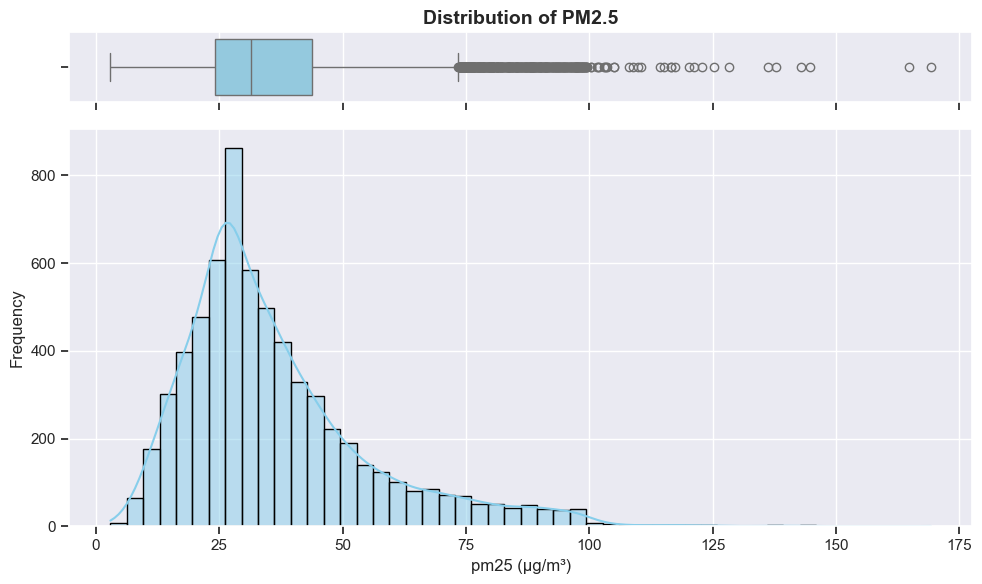
\includegraphics[width=0.8\textwidth]{figure/pm2.5.png}
    \caption{Phân phối nồng độ PM2.5 trong tập huấn luyện (Histplot và Boxplot)}
    \label{fig:pm25_dist}
\end{figure}
\begin{figure}[H]
    \centering
    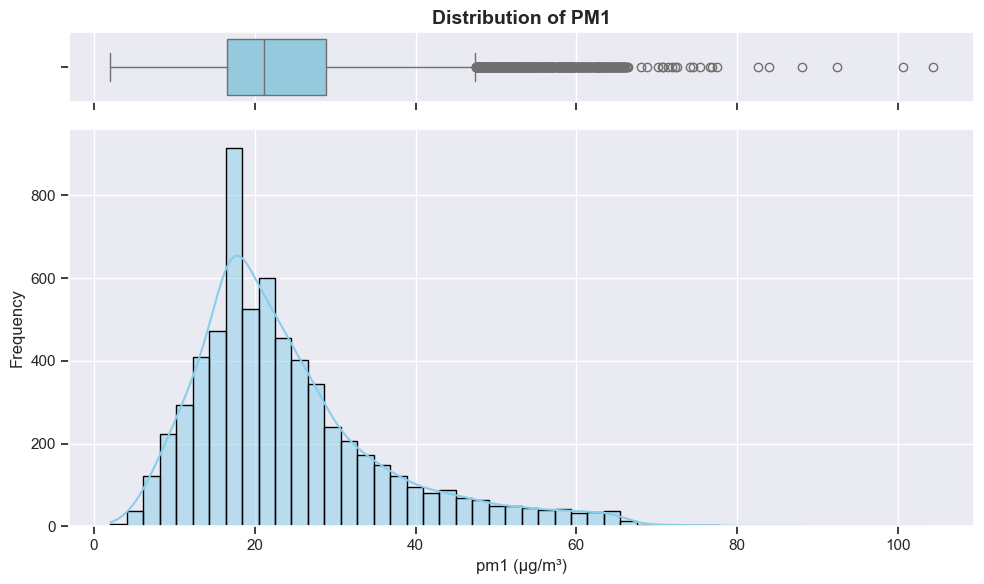
\includegraphics[width=0.8\textwidth]{figure/pm1.png}
    \caption{Phân phối nồng độ PM1 trong tập huấn luyện (Histplot và Boxplot)}
    \label{fig:pm1_dist}
\end{figure}
\begin{figure}[H]
    \centering
    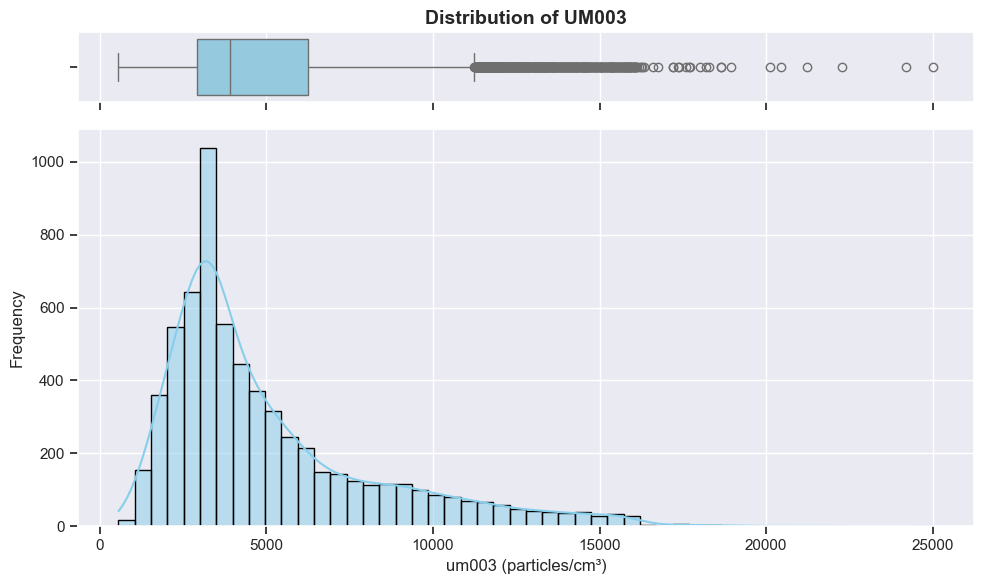
\includegraphics[width=0.8\textwidth]{figure/um003.png}
    \caption{Phân phối mật độ hạt bụi mịn kích thước $>$ 0.3$\mu m$ (UM003)}
    \label{fig:um003_dist}
\end{figure}
\begin{itemize}
    \item \textbf{PM2.5:} Giá trị đỉnh tập trung quanh ngưỡng 25--35 $\mu g/m^3$. Đáng chú ý, tập dữ liệu xuất hiện nhiều giá trị ngoại lai vượt mức 100 $\mu g/m^3$. Theo kết quả đối chiếu, các đỉnh ô nhiễm này thường tương ứng với các sự kiện khí tượng đặc biệt như nghịch nhiệt (\textit{Temperature Inversion}), khiến bụi mịn bị giữ lại ở tầng thấp không thể khuếch tán \cite{Le2024}.
    \item \textbf{PM1 và UM003:} Phân phối của hai biến này gần như đồng dạng với PM2.5. Sự tương quan chặt chẽ này khẳng định PM2.5 là thành phần chủ đạo bao hàm cả các hạt siêu mịn (PM1), đồng thời cho thấy việc sử dụng đồng thời cả ba chỉ số có thể dẫn đến hiện tượng đa cộng tuyến (\textit{Multicollinearity}) trong quá trình huấn luyện mô hình.
\end{itemize}
\subsubsection{Đối sánh dữ liệu khí tượng giữa hai nguồn trạm và vệ tinh}
Nghiên cứu thực hiện so sánh phân phối giữa cảm biến tại trạm (OpenAQ) và mô hình tái phân tích khí quyển (Open-Meteo) để đánh giá độ tin cậy.
\begin{figure}[H]
    \centering
    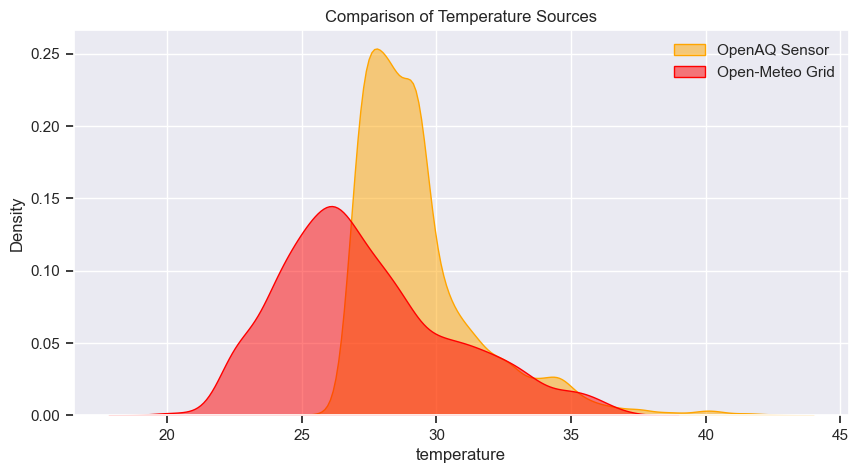
\includegraphics[width=0.8\textwidth]{figure/temperature.png}
    \caption{Đối sánh phân phối Nhiệt độ giữa nguồn OpenAQ và Open-Meteo}
    \label{fig:temp_comparison}
\end{figure}
\begin{figure}[H]
    \centering
    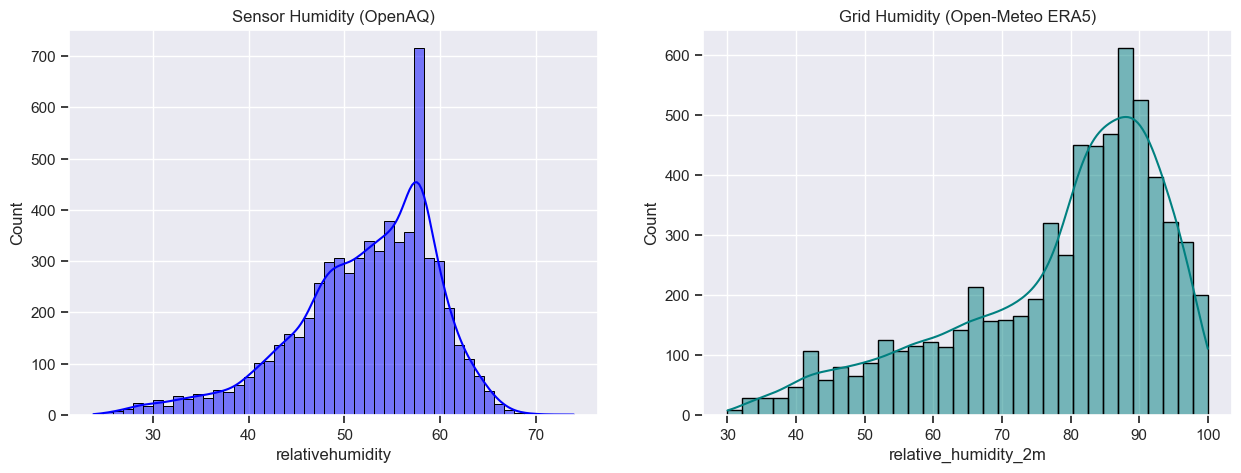
\includegraphics[width=0.8\textwidth]{figure/humidity.png}
    \caption{Đối sánh phân phối Độ ẩm giữa nguồn OpenAQ và Open-Meteo}
    \label{fig:humid_comparison}
\end{figure}
\begin{itemize}
    \item \textbf{Nhiệt độ (Temperature):} Cả hai nguồn đều thể hiện phân phối hai đỉnh (\textit{Bimodal}), phản ánh chu kỳ nhiệt ngày và đêm rõ rệt của khí hậu nhiệt đới. Tuy nhiên, nhiệt độ ghi nhận tại trạm (OpenAQ) thường cao hơn khoảng 1--2$^\circ$C so với dữ liệu vệ tinh, điều này có thể giải thích bởi hiệu ứng đảo nhiệt đô thị (\textit{Urban Heat Island}) tại vị trí đặt trạm thực tế.
    \item \textbf{Độ ẩm (Humidity):} Phân phối độ ẩm từ Open-Meteo có xu hướng mượt hơn (\textit{Smoothed}) so với dữ liệu trạm. Điều này cho thấy dữ liệu mô hình ERA5 đã trung bình hóa các biến động cực bộ, trong khi cảm biến tại chỗ phản ánh chính xác các biến động độ ẩm tức thời do các yếu tố môi trường xung quanh.
\end{itemize}

\subsubsection{Các đặc trưng khí quyển và động lực học}
Ngoài nhiệt độ và độ ẩm, các biến số khí quyển khác từ nguồn Open-Meteo cung cấp cái nhìn sâu sắc về các cơ chế khuếch tán và lắng đọng của bụi mịn.
\begin{figure}[H]
    \centering
    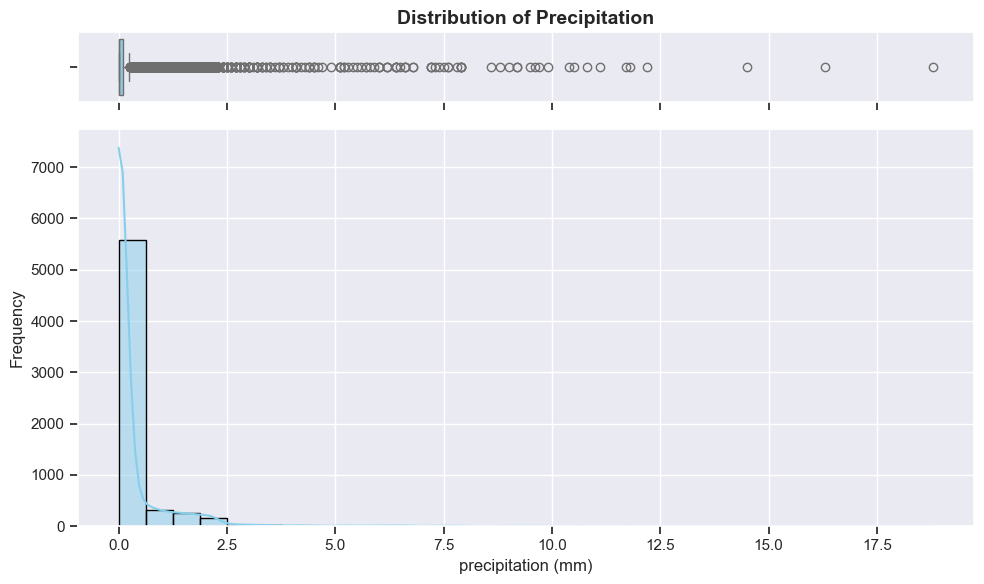
\includegraphics[width=0.8\textwidth]{figure/precipitation.png}
    \caption{Phân phối lượng mưa tích lũy theo giờ (Precipitation)}
    \label{fig:precip_dist}
\end{figure}
\begin{figure}[H]
    \centering
    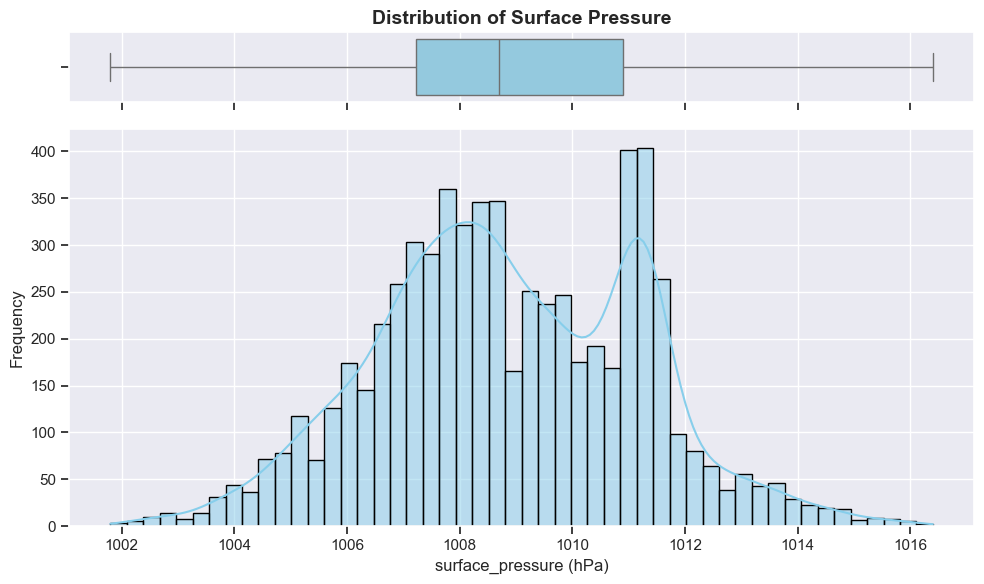
\includegraphics[width=0.8\textwidth]{figure/surface.png}
    \caption{Phân phối áp suất bề mặt (Surface Pressure)}
    \label{fig:pressure_dist}
\end{figure}
\begin{itemize}
    \item \textbf{Lượng mưa (Precipitation):} Tập dữ liệu cho thấy đặc tính phân phối rời rạc với tần suất các giờ không mưa chiếm ưu thế tuyệt đối. Lượng mưa là nhân tố then chốt thực hiện quá trình lắng đọng ướt (\textit{Wet deposition}), giúp loại bỏ các hạt PM2.5 ra khỏi khí quyển thông qua cơ chế rửa trôi \cite{Seinfeld2016}.
    \item \textbf{Áp suất bề mặt (Surface Pressure):} Biến số này biến động trong khoảng hẹp 1005--1015 hPa. Áp suất cao thường tương ứng với các trạng thái khí quyển ổn định, làm hạn chế sự khuếch tán thẳng đứng của các khối khí ô nhiễm \cite{Tai2010}.
\end{itemize}
\begin{figure}[H]
    \centering
    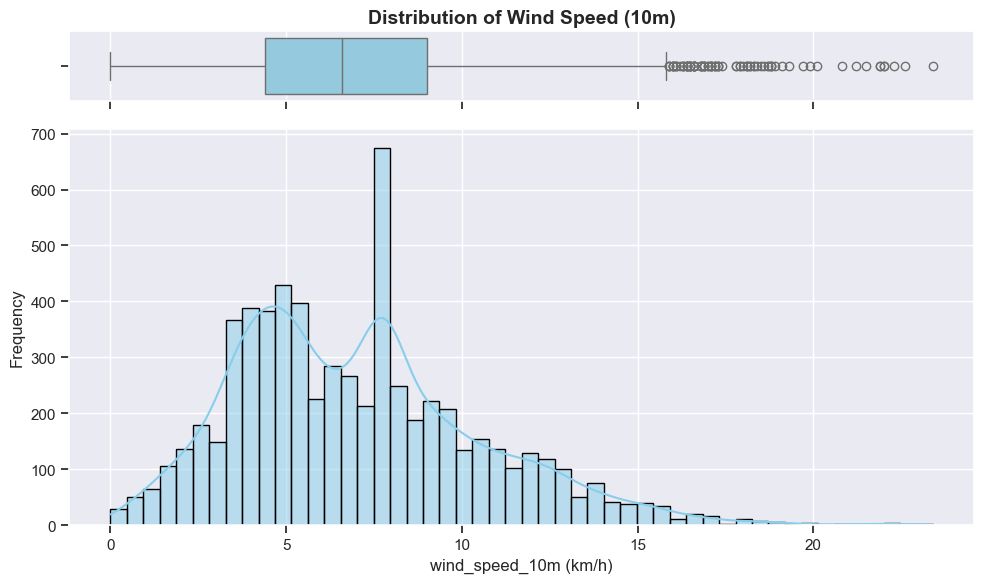
\includegraphics[width=0.8\textwidth]{figure/wind speed.png}
    \caption{Phân phối tốc độ gió tại độ cao 10m (Wind Speed)}
    \label{fig:wind_speed_dist}
\end{figure}
\begin{figure}[H]
    \centering
    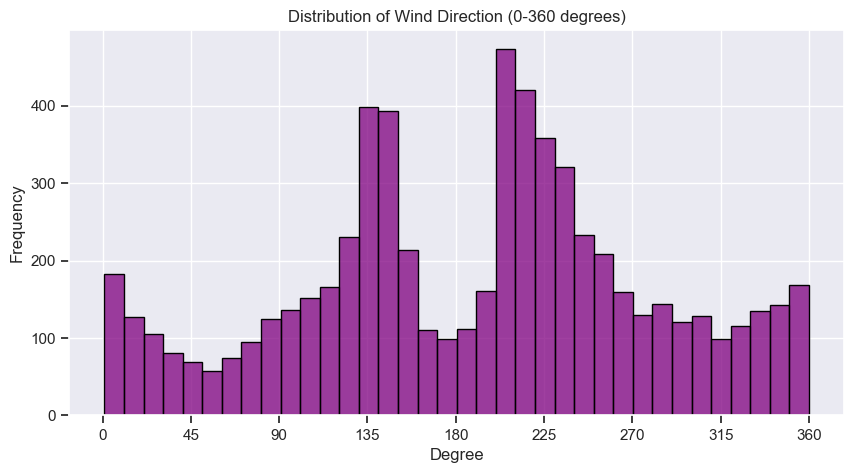
\includegraphics[width=0.6\textwidth]{figure/wind direction.png}
    \caption{Biểu đồ hoa gió thể hiện hướng và tốc độ gió thịnh hành (Wind Rose)}
    \label{fig:wind_rose}
\end{figure}
\begin{itemize}
    \item \textbf{Tốc độ và hướng gió:} Tốc độ gió tập trung chủ yếu ở dải 2--6 m/s. Tốc độ gió thấp thường dẫn đến hiện tượng đình trệ khí quyển (\textit{Stagnation}), là nguyên nhân chính gây ra các đợt tích tụ bụi mịn cục bộ. Biểu đồ hoa gió giúp xác định các hướng vận chuyển chất ô nhiễm chủ đạo từ các khu vực phát thải lân cận.
\end{itemize}
\begin{figure}[H]
    \centering
    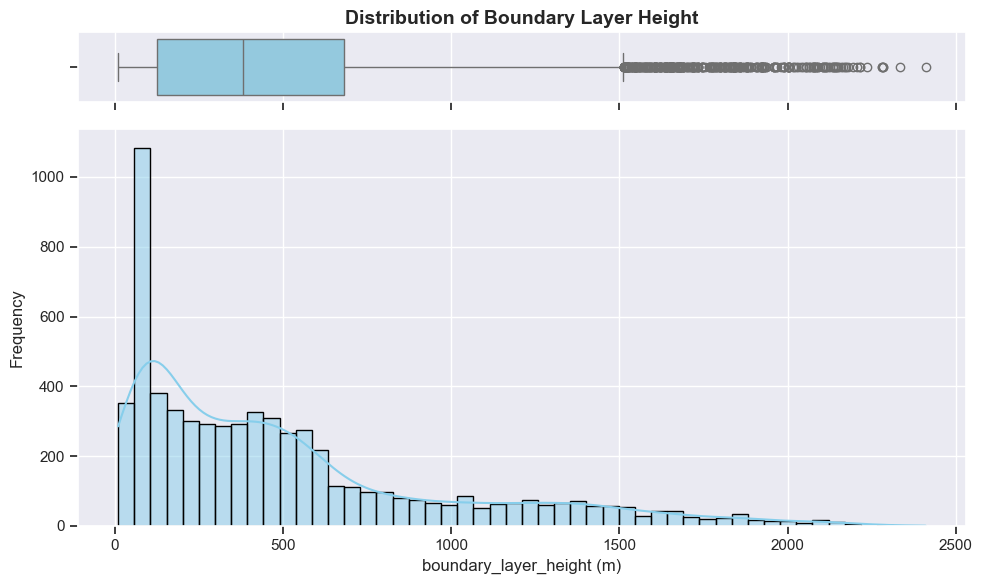
\includegraphics[width=0.8\textwidth]{figure/boundary layer height.png}
    \caption{Phân phối độ cao tầng biên khí quyển (Boundary Layer Height)}
    \label{fig:blh_dist}
\end{figure}
\begin{itemize}
    \item \textbf{Độ cao tầng biên (BLH):} BLH thể hiện sự biến thiên lớn giữa ngày và đêm. Một tầng biên nông (thấp) sẽ nén không gian thể tích khả dụng cho việc pha trộn bụi mịn, dẫn đến nồng độ quan trắc được tăng cao ngay cả khi cường độ nguồn thải không thay đổi \cite{Tai2010}.
\end{itemize}

\subsection{Phân tích nhị biến (Bivariate Analysis)}
Phân tích nhị biến tập trung vào việc làm rõ mối tương quan giữa nồng độ PM2.5 với các nhóm đặc trưng khí tượng và các yếu tố thời gian, từ đó định hình chiến lược lựa chọn đặc trưng (\textit{Feature Selection}) hiệu quả.
\subsubsection{Phân tích ma trận tương quan (Correlation Analysis)}
Hệ số tương quan Pearson được sử dụng để đánh giá mức độ liên kết tuyến tính giữa các cặp biến số trong tập dữ liệu.
\begin{figure}[H]
    \centering
    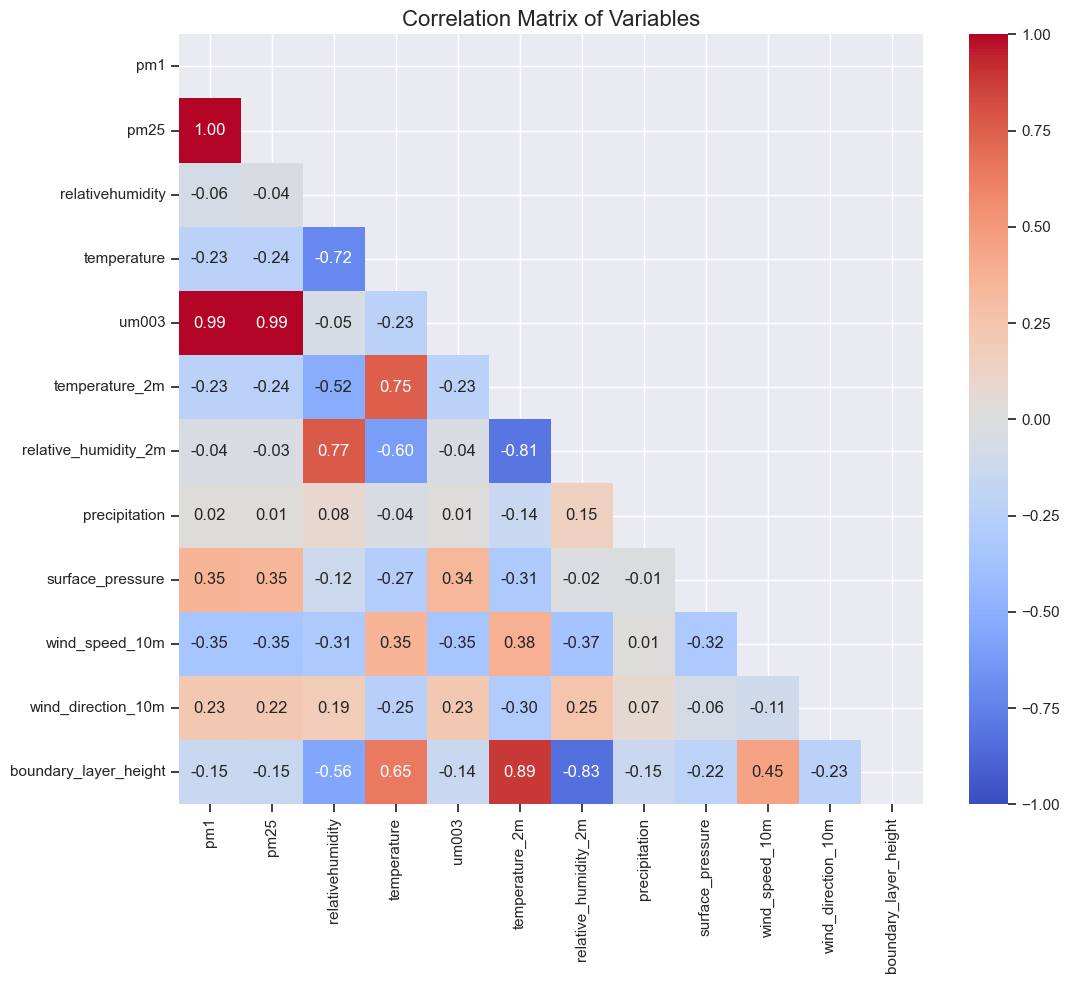
\includegraphics[width=0.9\textwidth]{figure/correlation.png}
    \caption{Ma trận tương quan Pearson giữa nồng độ bụi mịn và các biến khí tượng}
    \label{fig:correlation_heatmap}
\end{figure}
\begin{itemize}
    \item \textbf{Đa cộng tuyến giữa các kích cỡ hạt bụi:} PM2.5 thể hiện sự tương quan cực kỳ chặt chẽ ($r \approx 0.99$) với PM1 và UM003. Kết quả này gợi ý rằng các hạt bụi kích thước khác nhau có cùng nguồn gốc phát thải và cơ chế vận chuyển. Để tối ưu hóa mô hình và tránh hiện tượng đa cộng tuyến (\textit{Multicollinearity}), các biến PM1 và UM003 sẽ được loại bỏ trong giai đoạn tiền xử lý.
    \item \textbf{Tương quan với các biến ngoại sinh:} PM2.5 có tương quan nghịch rõ rệt với độ cao tầng biên (BLH) và tốc độ gió. Điều này phù hợp với lý thuyết về sự pha loãng chất ô nhiễm: khi gió mạnh và tầng biên cao, thể tích không khí để bụi mịn khuếch tán tăng lên, dẫn đến nồng độ quan trắc được giảm xuống \cite{Seinfeld2016}.
\end{itemize}
\subsubsection{Các quy luật biến động theo thời gian (Temporal patterns)}
Nồng độ bụi mịn tại khu vực nghiên cứu thể hiện các đặc tính mang tính chu kỳ rõ rệt, phản ánh sự tương tác giữa hoạt động của con người và các hiện tượng tự nhiên.
\begin{figure}[H]
    \centering
    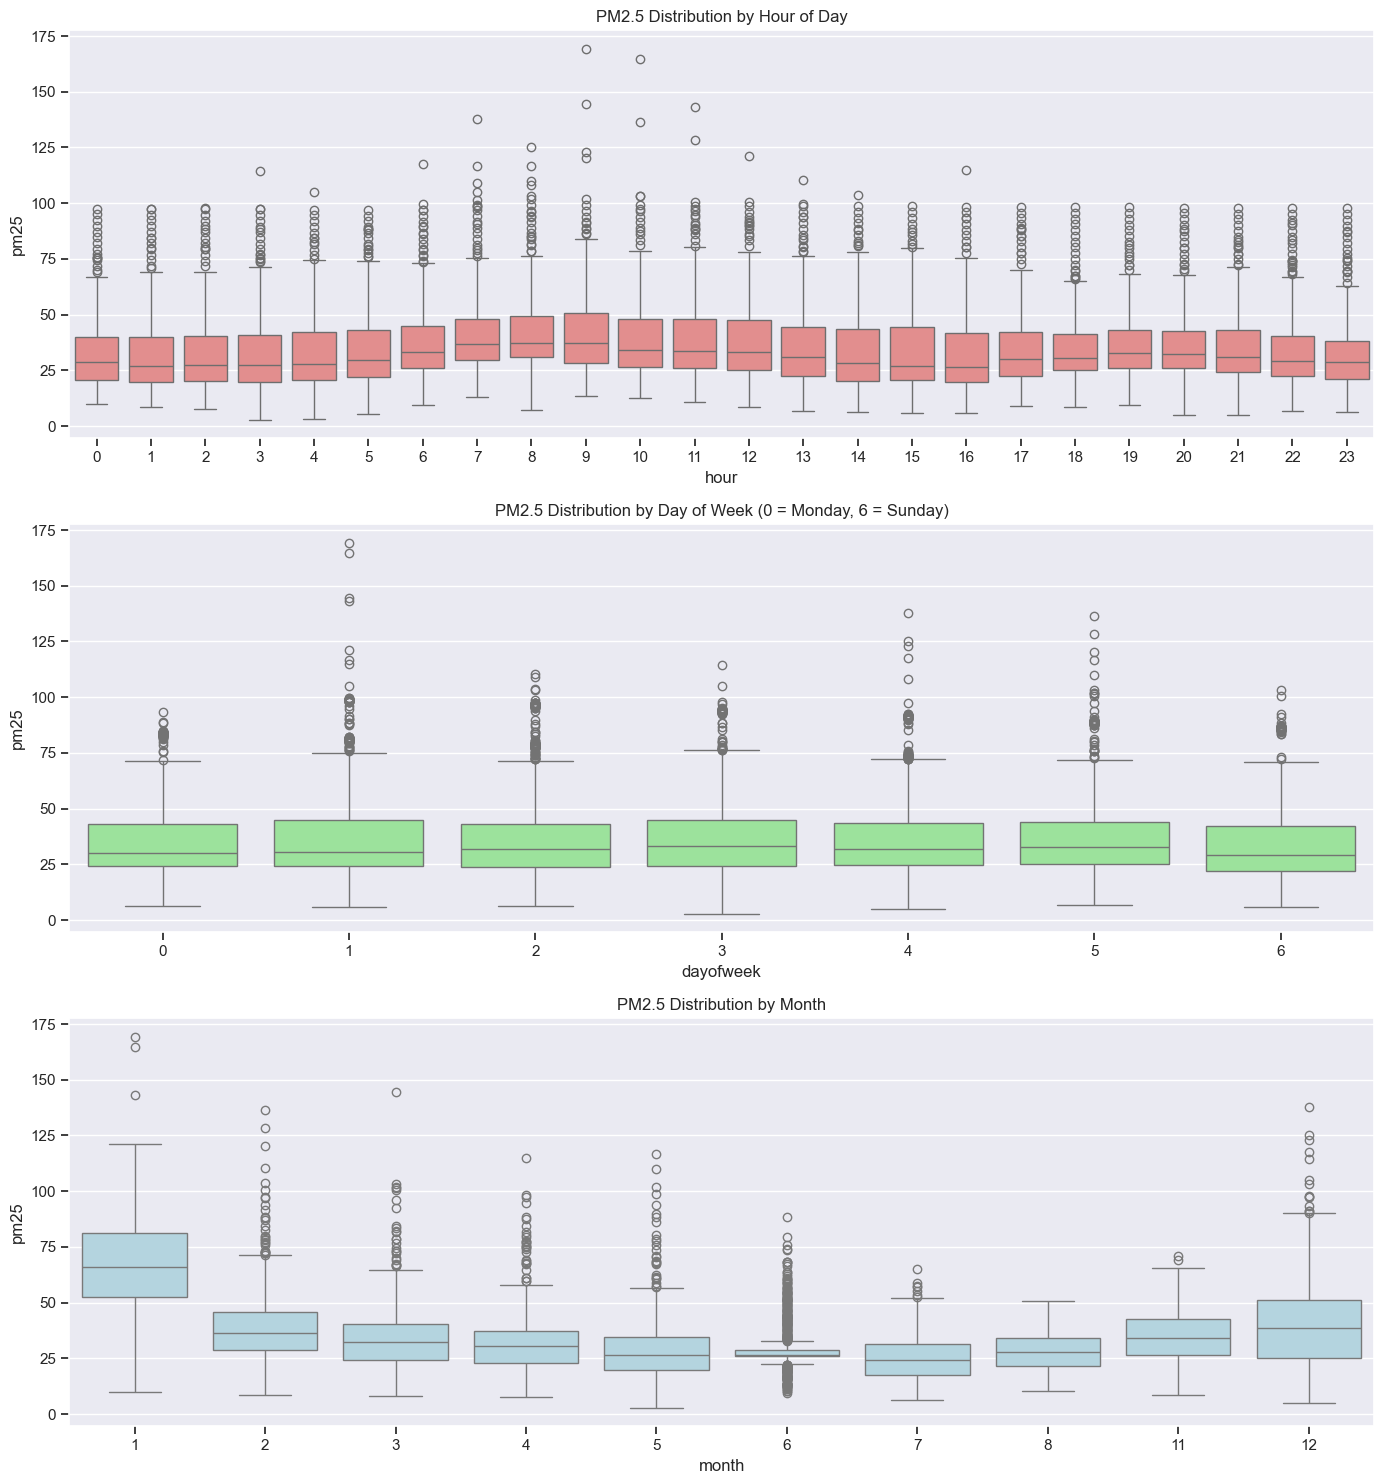
\includegraphics[width=0.9\textwidth]{figure/temporal pattern.png}
    \caption{Quy luật biến động thời gian của nồng độ PM2.5 trong ngày, trong tuần và trong tháng}
    \label{fig:temporal_patterns}
\end{figure}
\begin{itemize}
    \item \textbf{Chu kỳ giờ trong ngày (Diurnal Cycle):} Biểu đồ nồng độ theo giờ thể hiện đặc tính hai đỉnh (\textit{Bimodal}). Đỉnh thứ nhất xuất hiện vào khoảng 7h--9h sáng, trùng với giờ cao điểm giao thông. Đỉnh thứ hai cao và kéo dài hơn xuất hiện vào đêm khuya (sau 20h), thời điểm tầng biên khí quyển hạ xuống thấp nhất, gây ra hiện tượng tích tụ chất ô nhiễm gần bề mặt \cite{Tai2010}.
    \item \textbf{Chu kỳ ngày trong tuần (Weekly Cycle):} Nồng độ trung bình có xu hướng giảm vào các ngày cuối tuần, phản ánh sự sụt giảm trong lưu lượng giao thông công nghiệp và hoạt động xây dựng trong thành phố.
    \item \textbf{Biến động theo tháng (Monthly Variation):} Nồng độ bụi mịn thể hiện sự khác biệt rõ rệt giữa mùa khô và mùa mưa. Các tháng cuối năm và đầu năm (tháng 11, 12, 1) ghi nhận nồng độ cao vượt trội do điều kiện khí quyển ổn định và ít mưa. Ngược lại, các tháng giữa năm (tháng 6, 7, 8) có nồng độ thấp và ổn định hơn nhờ hiệu ứng rửa trôi của mưa \cite{Seinfeld2016}.
    \end{itemize}
\textit{Lưu ý:} Do quy trình EDA chỉ thực hiện trên tập huấn luyện (Train Only) bao gồm 60\% dữ liệu đầu tiên theo trục thời gian (từ tháng 11/2024 đến tháng 08/2025), nên các tháng 9 và tháng 10 không xuất hiện trong phân tích này. Việc giới hạn không gian phân tích trong tập Huấn luyện là cần thiết để đảm bảo tính khách quan cho quá trình tối ưu hóa mô hình sau này.

\subsubsection{Tương quan giữa nồng độ PM2.5 và các yếu tố khí tượng}
Việc phân tích các mối quan hệ nhị biến trực tiếp giữa bụi mịn và các điều kiện vật lý giúp hiểu rõ cơ chế khuếch tán và tích tụ tại địa phương.
\begin{figure}[H]
    \centering
    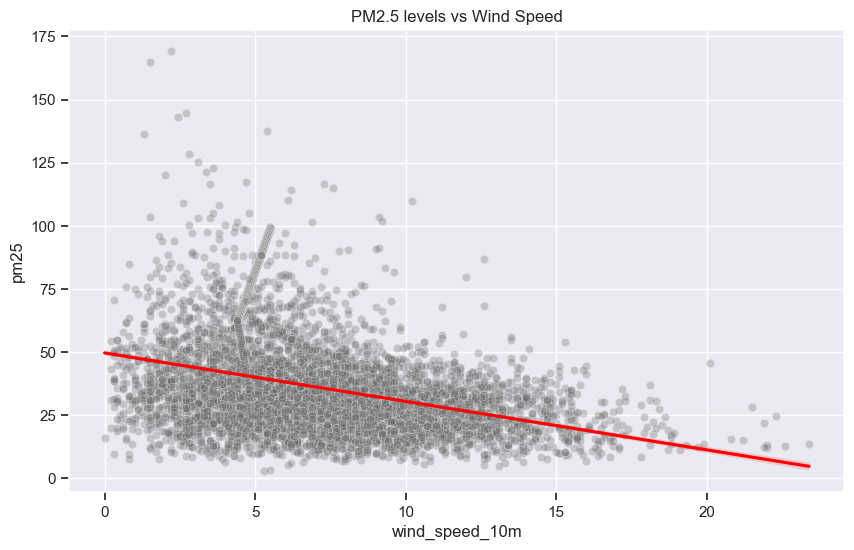
\includegraphics[width=0.8\textwidth]{figure/pm2.5 vs wind speed.png}
    \caption{Mối quan hệ nghịch biến giữa nồng độ PM2.5 và tốc độ gió}
    \label{fig:pm25_vs_windspeed}
\end{figure}
\begin{itemize}
    \item \textbf{PM2.5 và Tốc độ gió:} Kết quả thể hiện mối quan hệ nghịch biến rõ rệt. Khi tốc độ gió vượt ngưỡng 4 m/s, nồng độ PM2.5 giảm xuống mức thấp và ổn định. Điều này được giải thích bởi sự gia tăng năng lượng pha loãng và vận chuyển ngang của các khối khí ô nhiễm. Ngược lại, các điều kiện "lặng gió" ($<$ 1.5 m/s) là tiền đề cho các sự kiện tích tụ ô nhiễm nghiêm trọng do chất thải từ giao thông không thể phát tán \cite{Tai2010}.
\end{itemize}
\begin{figure}[H]
    \centering
    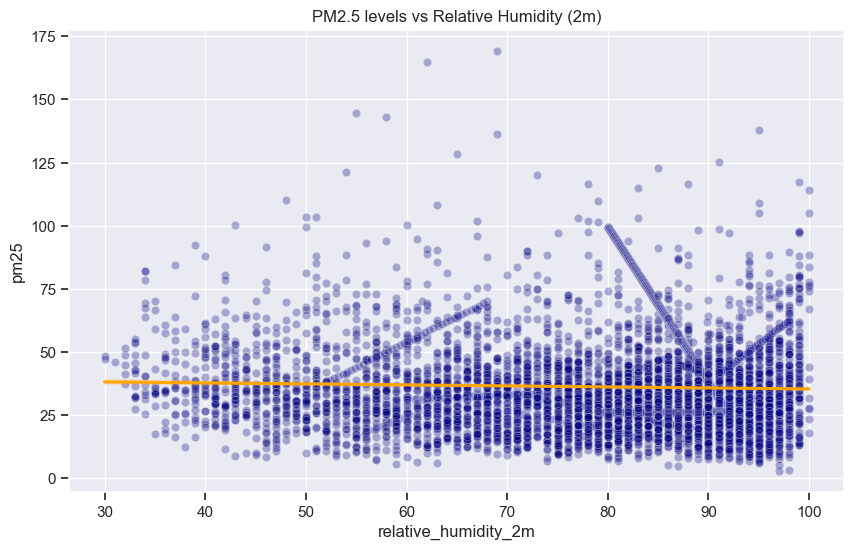
\includegraphics[width=0.8\textwidth]{figure/pm2.5 vs relative humidity.png}
    \caption{Phân tích biến thiên nồng độ PM2.5 theo độ ẩm tương đối}
    \label{fig:pm25_vs_humidity}
\end{figure}
\begin{itemize}
    \item \textbf{PM2.5 và Độ ẩm:} Mối quan hệ này có tính phức tạp và phụ thuộc vào ngưỡng. Trong dải độ ẩm từ 50\% đến 80\%, nồng độ PM2.5 có xu hướng tăng tỷ lệ thuận với độ ẩm do cơ chế tăng trưởng hút ẩm (\textit{Hygroscopic growth}), khiến các sol khí liên kết với hơi nước và tăng trọng lượng \cite{Seinfeld2016}. Tuy nhiên, ở các ngưỡng độ ẩm cực cao ($>$ 90\%), nồng độ thường giảm mạnh, phản ánh sự xuất hiện của mưa và quá trình rửa trôi khí quyển.
\end{itemize}
\begin{figure}[H]
    \centering
    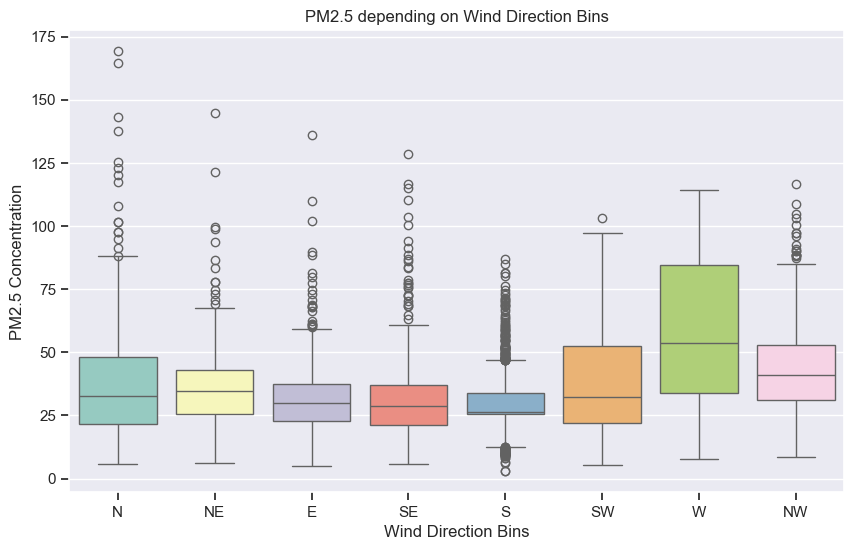
\includegraphics[width=0.7\textwidth]{figure/pm2.5 wind dir.png}
    \caption{Phân bổ nồng độ PM2.5 trung bình theo các hướng gió chính}
    \label{fig:pm25_by_wind_dir}
\end{figure}
\begin{itemize}
    \item \textbf{PM2.5 và Hướng gió:} Sự phân bổ nồng độ bụi theo hướng gió cho thấy tính bất đẳng hướng rõ rệt. Các hướng gió mang nồng độ cao thường tương ứng với các luồng khí thổi từ phía các khu công nghiệp phụ cận hoặc dọc theo các trục lộ giao thông huyết mạch của TP.HCM, chứng minh tầm quan trọng của nguồn phát thải liên tỉnh và liên vùng đối với chất lượng không khí đô thị.
\end{itemize}

\subsection{Phân tích đa biến (Multivariate Analysis)}
Giai đoạn cuối của quá trình EDA tập trung vào việc bóc tách các thành phần cấu trúc của chuỗi thời gian và nhận diện nguồn phát thải thông qua sự kết hợp giữa nồng độ chất ô nhiễm và động lực học khí quyển.
\subsubsection{Nhận diện hướng vận chuyển ô nhiễm (Pollution Rose)}
Biểu đồ hoa gió ô nhiễm (\textit{Pollution Rose}) tích hợp thông tin về nồng độ PM2.5, hướng gió và tần suất xuất hiện để xác định các hành lang vận chuyển chất ô nhiễm chủ đạo.
\begin{figure}[H]
    \centering
    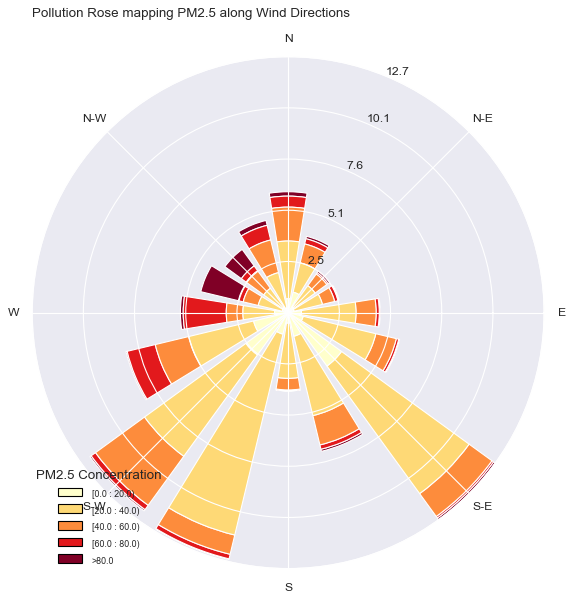
\includegraphics[width=0.7\textwidth]{figure/Pollution Rose.png}
    \caption{Biểu đồ Pollution Rose thể hiện nồng độ PM2.5 theo hướng gió}
    \label{fig:pollution_rose}
\end{figure}
Kết quả phân tích cho thấy các sự kiện ô nhiễm nồng độ cao (trên 80 $\mu g/m^3$) có tần suất xuất hiện lớn khi gió thổi từ các hướng Nam và Tây Nam. Điều này cho thấy ảnh hưởng mạnh mẽ của các nguồn thải từ các khu công nghiệp tập trung và hoạt động cảng biển phía Nam thành phố, đóng đóng vai trò là nguồn phát thải liên vùng quan trọng \cite{Le2024}.
\subsubsection{Phân rã chuỗi thời gian (Time-series Decomposition)}
Quá trình phân rã chuỗi thời gian giúp tách biệt các thành phần xu hướng, chu kỳ và nhiễu nhằm hiểu rõ cấu trúc nội tại của dữ liệu bụi mịn.
\begin{figure}[H]
    \centering
    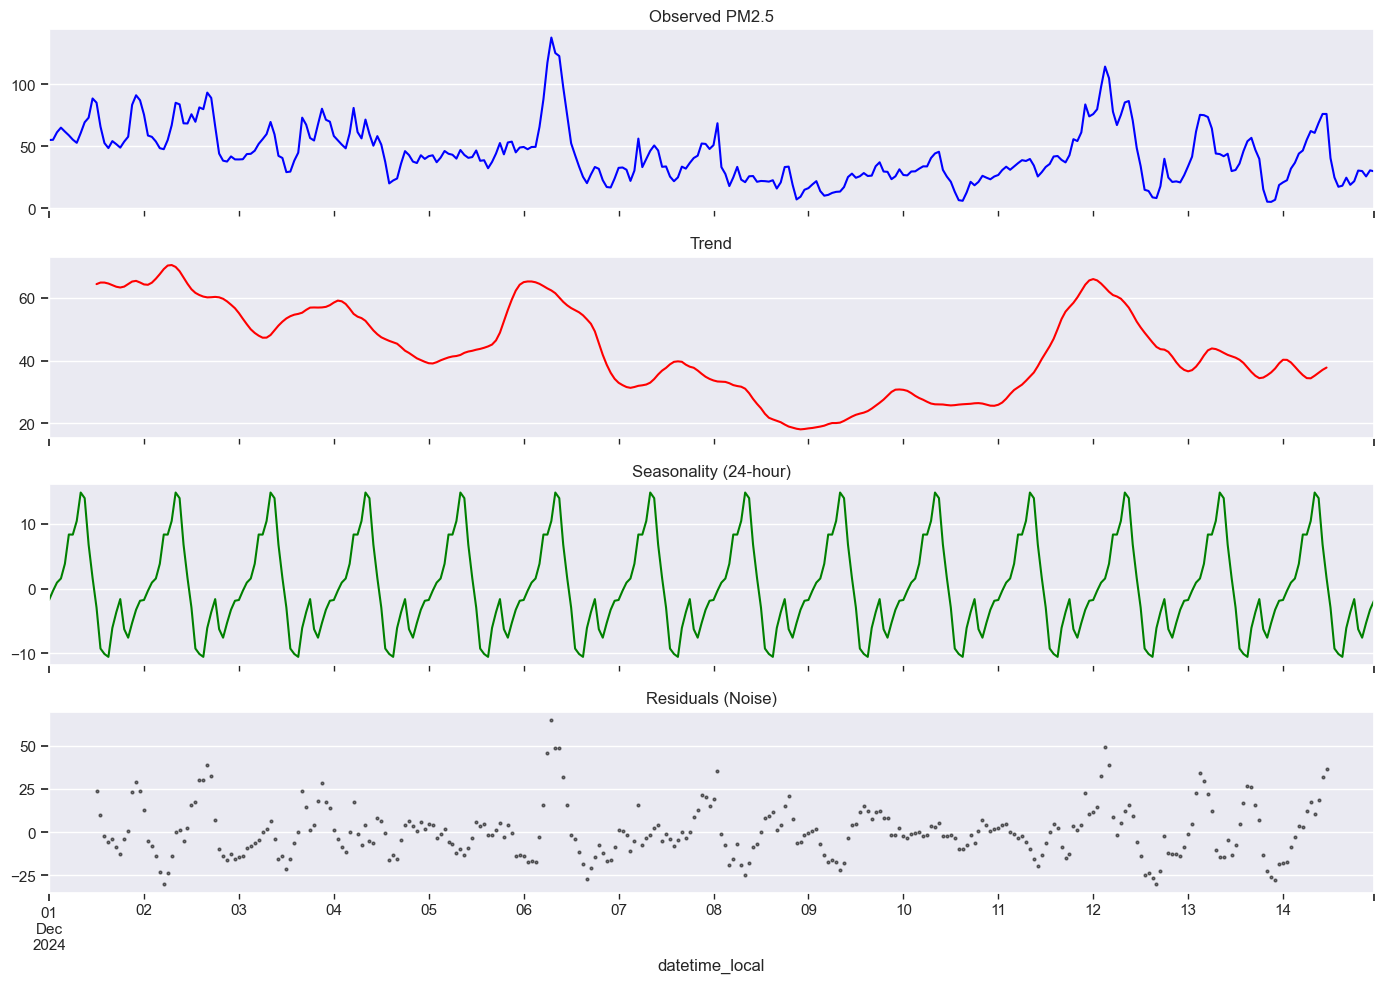
\includegraphics[width=1\textwidth]{figure/ts decompose.png}
    \caption{Phân rã chuỗi thời gian PM2.5 thành các thành phần Xu hướng, Chu kỳ và Nhiễu}
    \label{fig:ts_decomp}
\end{figure}
\begin{itemize}
    \item \textbf{Thành phần xu hướng (\textit{Trend}):} Thể hiện sự biến động dài hạn, phản ánh các tác động của điều kiện khí tượng vĩ mô và nhịp độ kinh tế xã hội.
    \item \textbf{Thành phần chu kỳ (\textit{Seasonality}):} Chu kỳ 24 giờ lặp lại rất ổn định, khẳng định sự chi phối tuyệt đối của hoạt động giao thông đô thị và sự co giãn của tầng biên khí quyển (BLH) đối với nồng độ bụi mịn tại bề mặt \cite{Tai2010}.
    \item \textbf{Thành phần nhiễu (\textit{Residuals}):} Đại diện cho các biến động ngẫu nhiên hoặc các sự kiện ô nhiễm cực đoan không mang tính chu kỳ.
\end{itemize}
\subsubsection{Phân tích tự tương quan (ACF và PACF)}
Việc đánh giá tính tự tương quan đóng vai trò nền tảng trong việc thiết lập các tham số cho các mô hình dự báo thống kê và học máy.
\begin{figure}[H]
    \centering
    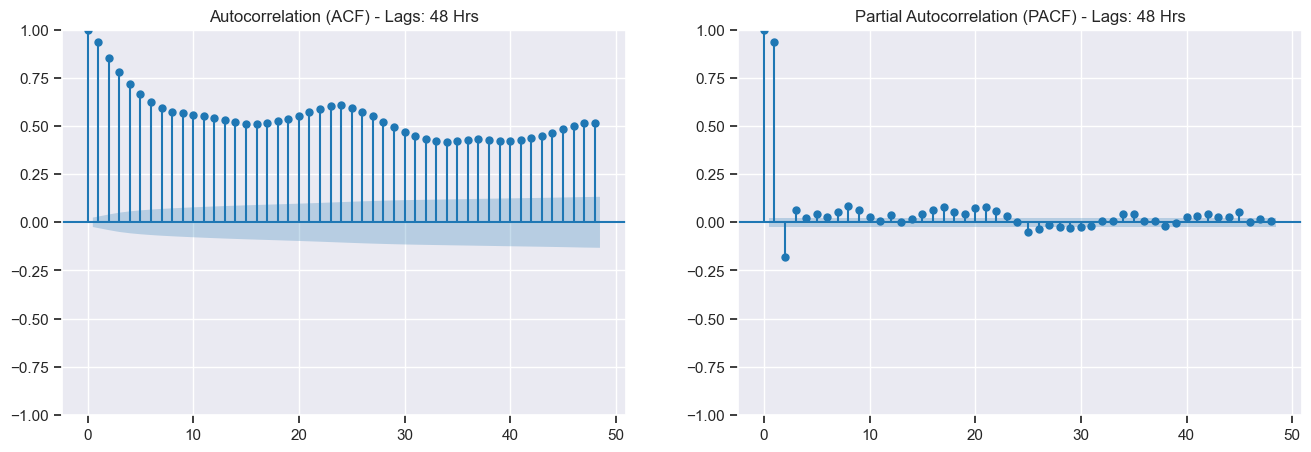
\includegraphics[width=1\textwidth]{figure/acf and pacf.png}
    \caption{Biểu đồ tự tương quan (ACF) và tự tương quan riêng phần (PACF) của chuỗi PM2.5}
    \label{fig:acf_pacf}
\end{figure}
\begin{itemize}
    \item \textbf{Tự tương quan (ACF):} Hàm ACF giảm chậm (\textit{Slow decay}) và có tính lặp lại sau mỗi 24 giờ. Điều này cho thấy chuỗi dữ liệu có tính "trì trệ" (\textit{Persistence}) rất cao, nghĩa là nồng độ bụi trong quá khứ có ảnh hưởng kéo dài đến các thời điểm tương lai.
    \item \textbf{Tự tương quan riêng phần (PACF):} PACF xuất hiện các hệ số có ý nghĩa thống kê tại các bậc trễ đầu tiên (Lag 1, 2). Kết quả này khẳng định cấu trúc tự hồi quy (\textit{Autoregressive}) mạnh mẽ của dữ liệu, là cơ sở để áp dụng các mô hình ARIMA hoặc các mạng học sâu như LSTM nhằm nắm bắt các phụ thuộc thời gian ngắn hạn và dài hạn \cite{Box2015}.
\end{itemize}

\subsubsection{Phân loại chất lượng không khí (AQI Categorization)}
Để đánh giá mức độ ảnh hưởng của nồng độ PM2.5 đối với sức khỏe cộng đồng, nghiên cứu thực hiện phân loại dữ liệu huấn luyện theo Quy chuẩn kỹ thuật quốc gia về môi trường của Việt Nam (VN\_AQI).
\begin{figure}[H]
    \centering
    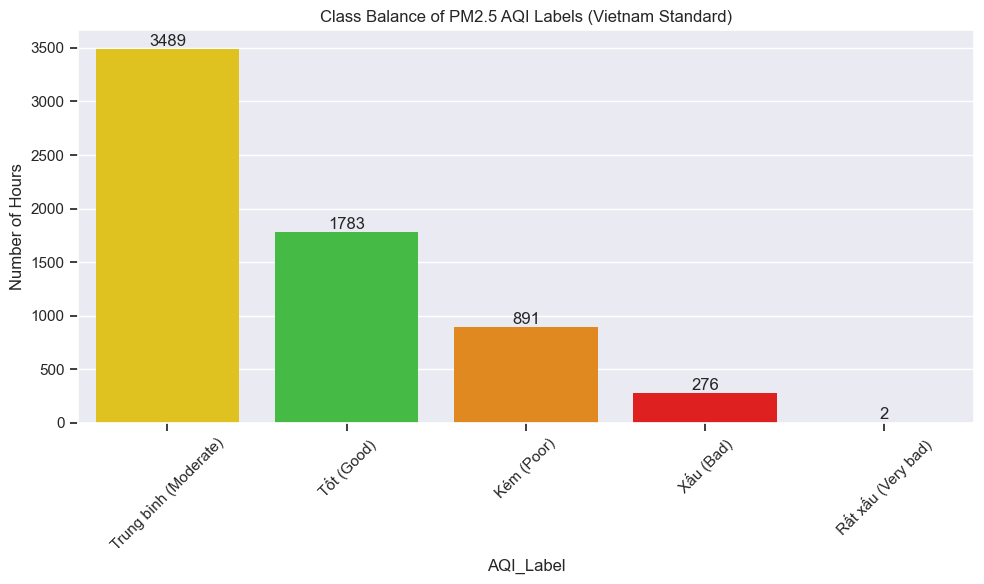
\includegraphics[width=0.8\textwidth]{figure/AQI.png}
    \caption{Phân bổ các mức chất lượng không khí (AQI) theo tiêu chuẩn Việt Nam trong tập huấn luyện}
    \label{fig:aqi_balance}
\end{figure}
Kết quả thống kê cho thấy nồng độ PM2.5 tại khu vực nghiên cứu phần lớn thời gian nằm ở ngưỡng "Trung bình" (Moderate - 3.489 giờ) và "Tốt" (Good - 1.783 giờ). Tuy nhiên, số lượng giờ quan trắc ở mức "Kém" (Poor) và "Xấu" (Bad) vẫn chiếm tỷ lệ đáng kể, khẳng định tính cấp thiết của việc dự báo sớm nhằm bảo vệ sức khỏe người dân \cite{Le2024}.
Đáng lưu ý, biểu đồ thể hiện sự mất cân bằng lớp (\textit{Class Imbalance}) cực kỳ nghiêm trọng, đặc biệt là ở mức "Rất xấu" (Very Bad) chỉ xuất hiện 2 mẫu. Sự khan hiếm của các dữ liệu ô nhiễm cực đoan trong tập huấn luyện tạo nên rào cản cho mô hình trong việc học các đặc trưng của những sự kiện hiếm gặp nhưng có tác động tiêu cực nhất \cite{Box2015}.

\subsection{Kết luận EDA}
Quá trình phân tích dữ liệu khám phá (EDA) trên tập huấn luyện đã cung cấp một bức tranh toàn diện về đặc tính của bụi mịn PM2.5 tại khu vực nghiên cứu, tạo tiền đề vững chắc cho việc xây dựng các mô hình dự báo. Những kết luận chính yếu từ chương này bao gồm:
\begin{itemize}
    \item \textbf{Đặc trưng thống kê và Mối quan hệ giữa các kích cỡ bụi:} Dữ liệu nồng độ bụi thể hiện dạng phân phối lệch phải mạnh với sự hiện diện thường xuyên của các giá trị ngoại lai cực đoan (\textit{outliers}), đòi hỏi các kỹ thuật chuẩn hóa mạnh mẽ trong giai đoạn tiền xử lý. Sự tương quan xấp xỉ tuyệt đối ($r \approx 0.99$) giữa PM2.5, PM1 và UM003 khẳng định tính đồng nhất trong cơ chế phát thải đô thị, đồng thời cho thấy việc tập trung dự báo PM2.5 là hướng tiếp cận đại diện tối ưu \cite{Le2024}.
    \item \textbf{Cơ chế chi phối của yếu tố khí tượng:} Thông qua phân tích nhị biến và đa biến, nghiên cứu xác định độ cao tầng biên (BLH) và tốc độ gió là hai nhân tố có ảnh hưởng nghịch biến mạnh mẽ nhất đến nồng độ bụi mịn. Phân tích \textit{Pollution Rose} đã nhận diện được các hành lang vận chuyển ô nhiễm chủ đạo từ hướng Nam và Tây Nam, cho thấy sự ảnh hưởng từ các khu vực phát thải công nghiệp liên vùng. Ngoài ra, vai trò của lượng mưa trong việc lắng đọng ướt cũng được làm rõ, giải thích sự sụt giảm nồng độ đáng kể trong các tháng mùa mưa \cite{Seinfeld2016}.
    \item \textbf{Tính chất chu kỳ và Cấu trúc thời gian:} Kết quả phân rã chuỗi thời gian (STL) và phân tích ACF/PACF khẳng định chuỗi dữ liệu PM2.5 mang tính chu kỳ 24 giờ ổn định và tính phụ thuộc quá khứ (\textit{Persistence}) cao. Đỉnh ô nhiễm \textit{bimodal} vào sáng sớm và đêm muộn trùng khớp với chu kỳ hoạt động giao thông và sự biến động của tầng biên khí quyển \cite{Tai2010}. Những đặc tính này gợi mở việc ứng dụng các mô hình học sâu có khả năng nắm bắt phụ thuộc thời gian như LSTM, GRU hoặc các mô hình thống kê SARIMAX tích hợp biến ngoại sinh.
    \item \textbf{Thách thức về mất cân bằng dữ liệu:} Biểu đồ phân bổ AQI theo tiêu chuẩn Việt Nam cho thấy sự mất cân bằng lớp cực kỳ nghiêm trọng. Việc các lớp "Xấu" và "Rất xấu" chiếm tỷ lệ mẫu rất thấp đặt ra thách thức về độ nhạy (\textit{Recall}) của mô hình. Điều này đòi hỏi các chiến lược huấn luyện đặc thù để đảm bảo khả năng cảnh báo chính xác các sự kiện ô nhiễm cực đoan \cite{Box2015}.
\end{itemize}
Tóm lại, những kết quả thu được từ EDA không chỉ mô tả thực trạng chất lượng không khí mà còn trực tiếp định hướng cho chiến lược lựa chọn đặc trưng (\textit{Feature Selection}) và thiết lập cấu trúc mô hình tối ưu sẽ được triển khai trong chương kế tiếp.

\section{Tiền xử lý dữ liệu (Preprocessing)}
Sau khi hiểu rõ bản chất dữ liệu qua bước EDA, nghiên cứu thiết lập một quy trình tiền xử lý (\textit{Preprocessing Pipeline}) có tính hệ thống cao. Do đặc thù của bài toán dự báo chuỗi thời gian (\textit{Time-series Forecasting}), trình tự các bước được thiết kế chặt chẽ nhằm bảo đảm tính toàn vẹn của dữ liệu và ngăn chặn hiện tượng rò rỉ thông tin (\textit{Data Leakage}). Quy trình bao gồm việc khởi tạo các đặc trưng liên tục trên toàn bộ chuỗi thời gian trước khi thực hiện phân tách tập dữ liệu và lựa chọn đặc trưng. Ngoài ra, tiền xử lý còn được nhánh hóa nhằm đáp ứng các yêu cầu kỹ thuật khác biệt giữa nhóm mô hình dạng cây ($\textit{Tree-based}$) và nhóm mô hình học sâu ($\textit{Deep Learning}$).
\subsection{Kỹ thuật đặc trưng (Feature Engineering)}
Việc xây dựng tập đặc trưng (\textit{Feature Pool}) là bước đầu tiên và quan trọng nhất, được thực hiện trên dãy số liệu liên tục nhằm đảm bảo các biến trễ (\textit{Lags}) và thống kê cửa sổ trượt (\textit{Rolling Windows}) không bị đứt gãy. Quy trình này tập trung vào việc mô hình hóa các quy luật vật lý và hành vi đô thị ảnh hưởng đến nồng độ bụi mịn PM2.5 thông qua các nhóm biến số sau:
\begin{enumerate}
    \item \textbf{Đặc trưng thời gian và bối cảnh đô thị:} Trích xuất các thành phần thời gian để mô hình hóa chu kỳ sinh hoạt và tác động của con người:
    \begin{itemize}
        \item \texttt{hour}, \texttt{day\_of\_week}, \texttt{month}: Các thành phần thời gian cơ bản mô tả chu kỳ ngày, tuần và năm.
        \item \texttt{is\_weekend}: Biến nhị phân phân loại ngày cuối tuần nhằm nắm bắt sự thay đổi nhịp độ giao thông công nghiệp.
        \item \texttt{is\_rush\_hour}: Xác định các khung giờ cao điểm tiêu biểu tại TP.HCM (\textit{7--9h và 17--19h}) gắn liền với phát thải giao thông nội đô.
        \item \texttt{is\_dry\_season}: Phân loại mùa tại miền Nam Việt Nam (\textit{tháng 11 đến tháng 4 năm sau}), giai đoạn thường ghi nhận nồng độ bụi cao do ít mưa và khí quyển ổn định.
    \end{itemize}
    \item \textbf{Mã hóa vòng lặp (Cyclic Encoding):} Biến đổi các đặc trưng có tính chu kỳ sang không gian lượng giác bằng hàm Sin và Cos:
    \begin{itemize}
        \item \texttt{hour\_sin}, \texttt{hour\_cos}: Mã hóa chu kỳ 24 giờ.
        \item \texttt{month\_sin}, \texttt{month\_cos}: Mã hóa chu kỳ 12 tháng, giúp duy trì tính liên tục (ví dụ: khoảng cách giữa tháng 12 và tháng 1), hỗ trợ hiệu quả cho các mạng nơ-ron học sâu.
    \end{itemize}
    \item \textbf{Động lực học và Vật lý khí tượng:} Mô hình hóa các cơ chế vận chuyển và lắng đọng chất ô nhiễm:
    \begin{itemize}
        \item \texttt{is\_raining}: Chỉ báo trạng thái có mưa dựa trên dữ liệu khí tượng.
        \item \texttt{hours\_since\_last\_rain}: Tính toán thời gian tích lũy kể từ lần mưa gần nhất để mô tả sự phục hồi nồng độ bụi sau khi bị rửa trôi bởi hiện tượng lắng đọng ướt.
        \item \texttt{wind\_u}, \texttt{wind\_v}: Thành phần vector hóa của gió (tốc độ và hướng) trên trục tọa độ, giúp mô tả chính xác hướng vận chuyển khối khí thay vì sử dụng độ đơn thuần.
        \item \texttt{wind\_condition}: Biến định tính phân loại các mức độ tĩnh lặng hoặc lưu động của không khí.
        \item \texttt{pressure\_trend\_3h}: Biến thiên áp suất trong 3 giờ gần nhất nhằm theo dõi sự ổn định hoặc xáo trộn của các hệ thống khí tượng bề mặt.
    \end{itemize}
    \item \textbf{Đặc trưng trễ (Lags) và Biến động (Differences):} Tận dụng đặc tính trì trệ (\textit{Persistence}) và dữ liệu quá khứ:
    \begin{itemize}
        \item \texttt{pm25\_lag\_[1, 2, 3, 6, 12, 24, 48, 72]}: Giá trị nồng độ bụi tại các bậc trễ khác nhau, cung cấp thông tin về trạng thái không khí trong tối đa 3 ngày trước thời điểm dự báo.
        \item \texttt{pm25\_diff\_1h}, \texttt{pm25\_diff\_24h}: Tốc độ thay đổi nồng độ bụi so với 1 giờ và 24 giờ trước đó nhằm nắm bắt quán tính của chuỗi thời gian.
    \end{itemize}
    \item \textbf{Thống kê cửa sổ trượt (Rolling Statistics):} Nắm bắt xu hướng nồng độ bụi qua các quy mô thời gian khác nhau (\textit{6h, 12h, 24h, 48h, 72h}):
    \begin{itemize}
        \item \texttt{pm25\_roll\_[window]\_mean}: Trung bình trượt, giúp loại bỏ nhiễu cục bộ và nhận diện nồng độ nền trong khu vực.
        \item \texttt{pm25\_roll\_[window]\_std}: Độ lệch chuẩn trượt, phản ánh mức độ biến động cường độ mạnh hay yếu của chất ô nhiễm trong từng giai đoạn.
    \end{itemize}
\end{enumerate}

\subsection{Phân chia dữ liệu (Train/Val/Test Split)}
Để đánh giá chính xác khả năng tổng quát hóa của các mô hình dự báo, nghiên cứu thực hiện phân tách tập dữ liệu theo trình tự thời gian nghiêm ngặt (\textit{Chronological Split}). Phương pháp này đảm bảo tuân thủ nguyên tắc thực tiễn trong dự báo chuỗi thời gian: mô hình chỉ được học từ dữ liệu quá khứ và kiểm tra trên dữ liệu tương lai, tránh hiện tượng rò rỉ dữ liệu (\textit{Data Leakage}).
Tập dữ liệu bao gồm 10.639 bản ghi được phân chia theo tỷ lệ kinh nghiệm \textbf{60\% -- 20\% -- 20\%} cho các giai đoạn huấn luyện, kiểm định và kiểm tra cuối cùng:
\begin{itemize}
    \item \textbf{Tập huấn luyện (Training Set):} Bao gồm 6.383 mẫu (chiếm 60\%), kéo dài từ ngày 22/11/2024 đến ngày 15/08/2025. Đây là tập dữ liệu nền tảng để các thuật toán học hỏi các quy luật biến động chu kỳ và tương quan khí tượng.
    \item \textbf{Tập kiểm định (Validation Set):} Bao gồm 2.128 mẫu (chiếm 20\%), kéo dài từ ngày 15/08/2025 đến ngày 12/11/2025. Tập này đóng vai trò quan trọng trong việc tinh chỉnh siêu tham số (\textit{Hyperparameter Tuning}) và lựa chọn mô hình tối ưu.
    \item \textbf{Tập kiểm tra (Testing Set):} Bao gồm 2.128 mẫu (chiếm 20\%), kéo dài từ ngày 12/11/2025 đến ngày 09/02/2026. Tập dữ liệu này được giữ hoàn toàn độc lập và chỉ được sử dụng để đánh giá hiệu năng thực tế của các mô hình trong giai đoạn cuối cùng.
\end{itemize}
Việc phân tách này cũng cho thấy tính thử thách của bài toán, khi tập Testing rơi vào giai đoạn cuối năm và đầu năm mới --- thời điểm đỉnh điểm của mùa khô tại TP.HCM với các sự kiện ô nhiễm không khí phức tạp nhất.

\subsection{Phân tích và Lựa chọn đặc trưng (Feature Selection)}
Với một tập hợp đặc trưng phong phú được khởi tạo, nghiên cứu tiếp tục thực hiện quy trình lựa chọn đặc trưng (\textit{Feature Selection}) nhằm tối ưu hóa không gian tham số và giảm thiểu rủi ro quá khớp. Để đảm bảo tính khách quan, mọi quyết định lựa chọn đều dựa trên các phân tích thống kê thực hiện trên tập Huấn luyện.
\subsubsection{Loại bỏ các đặc trưng dựa trên kiến thức miền và EDA}
Một số nhóm đặc trưng được loại bỏ dựa trên các phân tích định lượng ở chương trước nhằm tinh gọn tập dữ liệu:
\begin{itemize}
    \item \textbf{Đa cộng tuyến và rò rỉ thông tin:} Loại bỏ \texttt{pm1} và \texttt{um003} do tương quan gần như tuyệt đối với biến mục tiêu ($r \approx 0.99$). Việc giữ lại các biến này có thể dẫn đến hiện tượng đa cộng tuyến (\textit{Multicollinearity}), khiến mô hình đưa ra các dự báo dựa trên nồng độ hạt thay vì học các quy luật vận chuyển hạt bụi.
    \item \textbf{Dữ liệu nhiễu và dư thừa:} Các biến khí tượng từ trạm OpenAQ (\texttt{temperature}, \texttt{relativehumidity}) bị loại bỏ do trùng lặp với nguồn Open-Meteo nhưng chứa nhiều nhiễu cảm biến cục bộ. 
    \item \textbf{Biến đổi định hướng:} \texttt{wind\_direction\_10m} bị loại bỏ để ưu tiên sử dụng các thành phần vector \texttt{wind\_u} và \texttt{wind\_v}, giúp giải quyết vấn đề không liên tục của vòng chia độ.
\end{itemize}
\subsubsection{Chiến lược xếp hạng đặc trưng lai (Hybrid Ranking Strategy)}
Nghiên cứu áp dụng phương pháp xếp hạng tầm quan trọng của các đặc trưng thông qua sự kết hợp giữa hai mô hình học máy: \textbf{Random Forest} (dựa trên mức giảm \textit{Impurity}) và \textbf{XGBoost} (dựa trên thông tin \textit{Gain}). 
Do mỗi mô hình có cơ chế tính toán và thang đo tầm quan trọng khác nhau, nghiên cứu thực hiện chuẩn hóa thứ tự ưu tiên của từng mô hình bằng kỹ thuật Min--Max trước khi tính toán \textbf{Thứ hạng trung bình (Mean Rank)}. Các đặc trưng có giá trị \textit{Mean Rank} thấp nhất (tương ứng với độ quan trọng cao nhất) sẽ được ưu tiên lựa chọn.
\subsubsection{Lựa chọn tập K-đặc trưng và Bảo lưu các biến trễ then chốt}
Quy trình lựa chọn cuối cùng được thiết lập theo cơ chế \textbf{Top-K + Forced Inclusion}:
\begin{enumerate}
    \item Lựa chọn \textbf{Top-25} đặc trưng có thứ hạng trung bình tốt nhất từ phân tích trên.
    \item Áp dụng cơ chế bảo lưu (\textit{Forced Inclusion}) để đảm bảo sự hiện diện của các biến trễ PACF quan trọng gồm \texttt{pm25\_lag\_1}, \texttt{pm25\_lag\_2} và \texttt{pm25\_lag\_24}. Đây là các biến mang thông tin về "bộ nhớ" ngắn hạn và chu kỳ ngày đêm của chuỗi thời gian đã được khẳng định qua bước EDA.
\end{enumerate}

Kết quả phân tích tầm quan trọng của các đặc trưng thông qua mô hình Random Forest và XGBoost đã mang lại những nhận định quan trọng phản ánh bản chất của dữ liệu:
\begin{figure}[H]
    \centering
    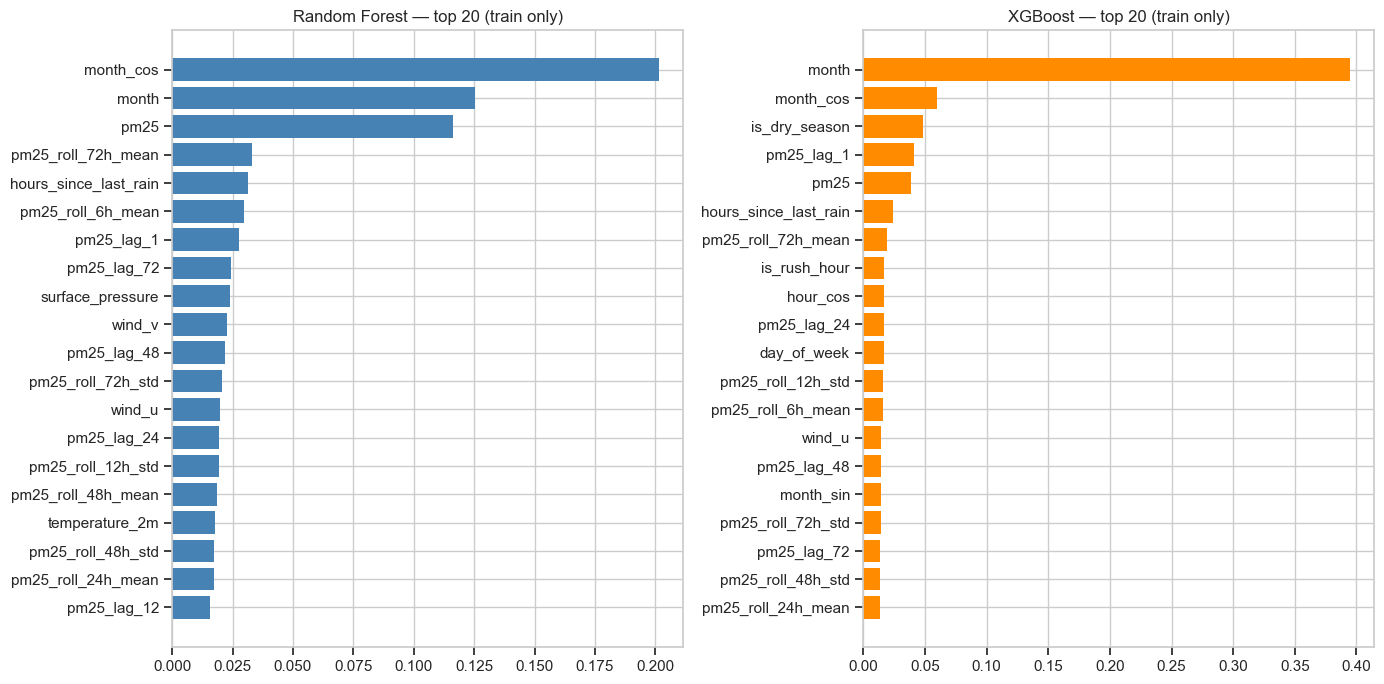
\includegraphics[width=1\textwidth]{figure/xgboost_rf.png}
    \caption{So sánh tầm quan trọng của các đặc trưng giữa Random Forest và XGBoost}
    \label{fig:feat_imp_comp}
\end{figure}
\begin{itemize}
    \item \textbf{Sự thống trị của tính mùa vụ:} Các biến \texttt{month} và \texttt{month\_cos} đứng đầu bảng xếp hạng ở cả hai mô hình. Điều này khẳng định chu kỳ năm và sự phân hóa mùa khô/mưa là nhân tố then chốt chi phối nồng độ PM2.5 tại khu vực nghiên cứu.
    \item \textbf{Tính trì trệ của chuỗi thời gian:} Nồng độ hiện tại (\texttt{pm25}) và các biến trễ gần nhất (\texttt{pm25\_lag\_1}) giữ thứ hạng rất cao, minh chứng cho tính tự tương quan mạnh mẽ của nồng độ chất ô nhiễm.
    \item \textbf{Vai trò của các yếu tố vật lý:} Đặc trưng \texttt{hours\_since\_last\_rain} xuất hiện trong nhóm 5 đặc trưng quan trọng nhất theo xếp hạng tổng hợp. Điều này cho thấy mô hình đã nắm bắt thành công cơ chế "rửa trôi" của mưa và sự tích lũy trở lại của bụi mịn. Ngoài ra, các thành phần vector gió (\texttt{wind\_u}, \texttt{wind\_v}) cũng đóng góp đáng kể cho việc giải thích hướng phát tán ô nhiễm.
    \item \textbf{Hiệu quả của đặc trưng cửa sổ trượt:} Các biến trung bình trượt (\texttt{pm25\_roll\_72h\_mean}, \texttt{pm25\_roll\_6h\_mean}) có thứ hạng cao, giúp mô hình nhận diện được xu hướng nồng độ nền (\textit{Background concentration}) thay vì chỉ dựa vào các giá trị tức thời có độ nhiễu cao.
\end{itemize}
\begin{figure}[H]
    \centering
    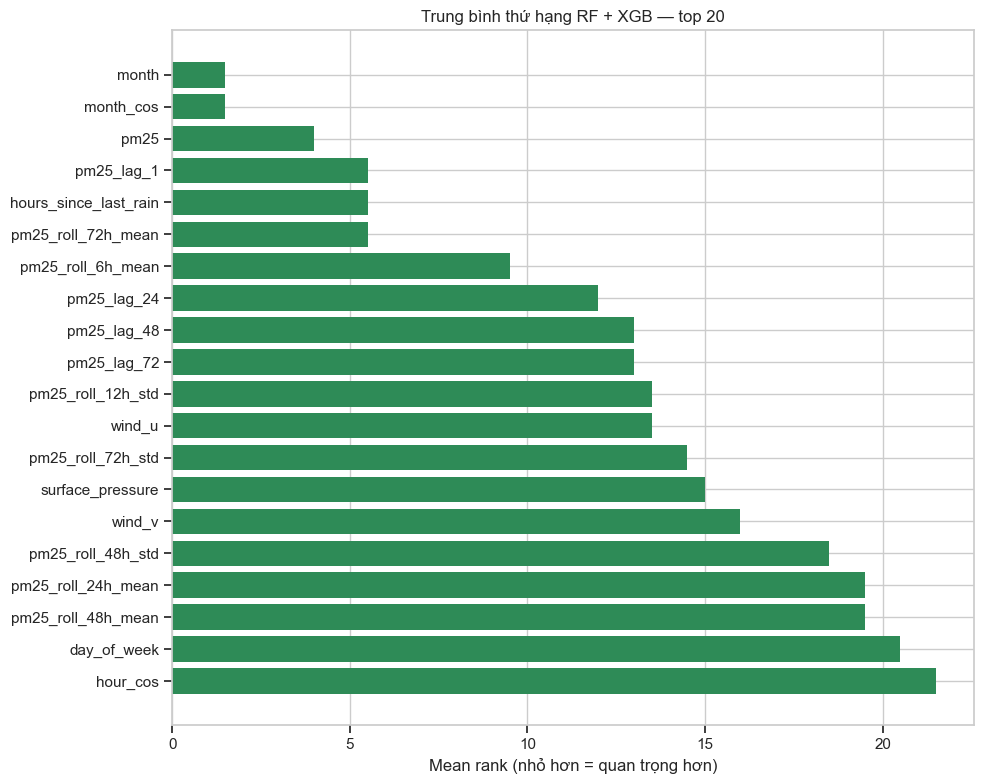
\includegraphics[width=0.85\textwidth]{figure/top20.png}
    \caption{Top 20 đặc trưng quan trọng nhất dựa trên Thứ hạng trung bình (Mean Rank)}
    \label{fig:mean_rank}
\end{figure}
Việc kết hợp đa dạng các nhóm đặc trưng từ thời gian, khí lượng đến các thông số chuỗi thời gian đảm bảo tập dữ liệu đầu vào có đầy đủ thông tin để mô hình thực hiện dự báo trong các điều kiện khí quyển biến động.

\subsection{Biến đổi và Chuẩn hóa dữ liệu (Scaling \& Transformation)}
Bước cuối cùng trong quy trình tiền xử lý là chuẩn hóa dữ liệu nhằm đáp ứng các yêu cầu kỹ thuật khắt khe của nhóm mô hình học sâu và mô hình thống kê. Khác với nhóm mô hình dạng cây có đặc tính không nhạy cảm với thang đo, các mạng nơ-ron học sâu (như LSTM, GRU) đòi hỏi dữ liệu đầu vào phải được biến đổi về một không gian phân phối ổn định để tối ưu hóa quá trình hội tụ của thuật toán luyện.
\begin{enumerate}
    \item \textbf{Biến đổi Logarit (Log-Transformation):} Do nồng độ PM2.5 có phân phối lệch phải mạnh với nhiều giá trị ngoại lai, nghiên cứu áp dụng hàm biến đổi \texttt{log1p} ($y = \ln(1+x)$) cho biến mục tiêu và toàn bộ nhóm đặc trưng có liên quan (\texttt{pm25}, các biến trễ, trung bình trượt). Kỹ thuật này giúp ổn định phương sai (\textit{Variance Stabilization}) và thu hẹp tầm ảnh hưởng của các giá trị ô nhiễm cực đoan, giúp mô hình nắm bắt tốt hơn các quy luật dài hạn.
    \item \textbf{Chuẩn hóa Z-score (Standardization):} Toàn bộ ma trận đặc trưng sau khi biến đổi logarit được đưa qua bộ chuẩn hóa \textit{StandardScaler}. Kỹ thuật này đưa dữ liệu về dạng có trung bình bằng 0 và độ lệch chuẩn bằng 1. Điều này đảm bảo rằng các trọng số trong mô hình được cập nhật đồng đều cho tất cả các nhóm biến số, tránh việc các biến khí tượng (thang đo nhỏ) bị lấn át bởi các biến nồng độ (thang đo lớn).
    \item \textbf{Nguyên tắc ngăn chặn rò rỉ và Khả năng hoàn tác:} Bộ chuẩn hóa chỉ được tính toán (\textit{fit}) duy nhất trên tập Huấn luyện. Các tham số thu được được bảo lưu để thực hiện quy trình chuyển đổi (\textit{transform}) cho các tập dữ liệu còn lại. Đồng thời, các tham số này cũng được sử dụng cho quá trình hoàn tác (\textit{Inverse Transformation}) bằng hàm \texttt{expm1} để đưa kết quả dự báo từ không gian logarit trở lại thang đo nồng độ gốc ($\mu g/m^3$) phục vụ giai đoạn đánh giá hiệu năng chính xác.
\end{enumerate}
Tóm lại, thông qua quy trình tiền xử lý dữ liệu có hệ thống từ xây dựng đặc trưng đến chuẩn hóa chuyên sâu, nghiên cứu đã thiết lập được một nền tảng dữ liệu vững chắc, sẵn sàng cho giai đoạn huấn luyện và so sánh hiệu năng các mô hình dự báo trong các chương tiếp theo.